\documentclass{article} 
\usepackage{tikz} 
\begin{document} 
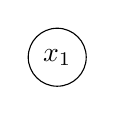
\begin{tikzpicture}[main/.style = {draw, circle}] 
\node[main] (1) {$x_1$}; 
\end{tikzpicture} 
\end{document}

\documentclass{article} 
\usepackage{tikz} 
\begin{document} 
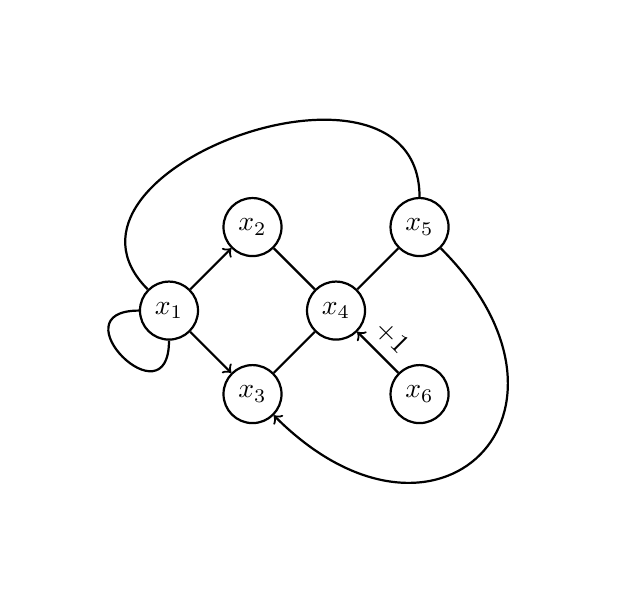
\begin{tikzpicture}[node distance={15mm}, thick, main/.style = {draw, circle}] 
\node[main] (1) {$x_1$}; 
\node[main] (2) [above right of=1] {$x_2$}; 
\node[main] (3) [below right of=1] {$x_3$}; 
\node[main] (4) [above right of=3] {$x_4$}; 
\node[main] (5) [above right of=4] {$x_5$}; 
\node[main] (6) [below right of=4] {$x_6$}; 
\draw[->] (1) -- (2); 
\draw[->] (1) -- (3); 
\draw (1) to [out=135,in=90,looseness=1.5] (5); 
\draw (1) to [out=180,in=270,looseness=5] (1); 
\draw (2) -- (4); 
\draw (3) -- (4); 
\draw (5) -- (4); 
\draw[->] (5) to [out=315, in=315, looseness=2.5] (3); 
\draw[->] (6) -- node[midway, above right, sloped, pos=1] {+1} (4); 
\end{tikzpicture} 
\end{document}

\documentclass{article}
\usepackage{neuralnetwork}
\begin{document}
\begin{neuralnetwork}
\newcommand{\x}[2]{$x_#2$}
\newcommand{\y}[2]{$y_#2$}
\newcommand{\h}[2]{$h_#2$}
\newcommand{\w}[4] {$w_{#2,#4}$}
\setdefaultlinklabel{\w}
\inputlayer[count=3, bias=false, text=\x]
\hiddenlayer[count=2, text=\h] 
\foreach \n in {1,...,3}{
    \foreach \m in {1,2}{
        \link[style={}, labelpos=near start, from layer=0, from node=\n, to layer=1, to node=\m]
    }
}
\outputlayer[count=1, text=\y] \linklayers
\end{neuralnetwork}
\end{document}



